\documentclass[main.tex]{subfiles}
% 速度和加速度
\begin{document}
在给定标架$\left(\mathcal{E},\phi\right)$下,设物体$B$在两时刻$t_1,t_2\in\mathbb{R}$下的构型分别为
\[\Omega_{t_1}=\kappa_{t_1}\left(B\right),\quad\Omega_{t_2}=\kappa_{t_2}\left(B\right)\]
则复合映射
\[\mu_{t_1\to t_2}:\Omega_{t_1}\rightarrow\Omega_{t_2},\quad\mu_{t_1\to t_2}=\kappa_{t_2}\circ\kappa_{t_1}^{-1}\]
称为物体$B$由$t_1$到$t_2$的\emph{形变(deformation)}。我们规定形变映射是可逆的;通常情况下还是任意所需阶光滑的。

\begin{figure}[ht]
    \centering
    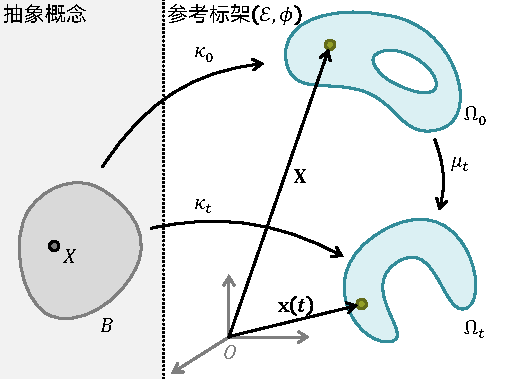
\includegraphics{images/III.6.1.pdf}
    \caption{物体$B$是物质点$X,Y,\dots$的集合,它只有在发生某种运动时,才能形成一系列物理事件,并在我们所选定的参考标架$\left(\mathcal{E},\phi\right)$下的欧几里得空间中表现出来。在参考时刻$t_0$,置放映射$\kappa_0$将物体$B$的每一物质点$X$映射为参考构型$\Omega_0$中的一点$\mathbf{X}$。在当前时刻$t$,置放映射$\kappa_t$将同一物质点$X\in B$映射为当前构型$\Omega_t$中的一点$\mathbf{x}\left(t\right)$。观察者只能观测到从参考构型到当前构型的变化,由形变映射$\mu_t=\kappa_t\circ\kappa_0^{-1}$描述。}
    \label{fig:III.6.1}
\end{figure}

如图\ref{fig:III.6.2}所示,我们常选定一个固定的时刻$t_0\in\mathbb{R}$作为\emph{参考时刻(reference instant)},$t_0$时物体$B$的构型$\Omega_0$称该物体的\emph{参考构型(reference configuration)},任一时刻$t$下物体$B$的构型称为\emph{当前构型(current configuration)}。在默认选定了参考构型的讨论中,我们依照以下记号惯例:
\begin{itemize}
    \item 物体$B$的物质点为$X,Y,\cdots\in B$
    \item 参考构型的位置向量:$\mathbf{X}=\kappa_0\left(X\right),\mathbf{Y}=\kappa_0\left(Y\right),\cdots\in\Omega_o$
    \item 当前构型的位置向量:$\mathbf{x}\left(t\right)=\kappa_t\left(X\right)=\mu_t\left(\mathbf{X}\right),\mathbf{y\left(t\right)}=\kappa_t\left(Y\right)=\mu_t\left(\mathbf{Y}\right),\cdots\in\Omega_t$
\end{itemize}
在上列记法中,使用同一字母,表示来自同一物质点。置放映射的像本应是欧几里得空间的点,使用向量来表示置放映射的像,是指它在基本坐标系下的位置向量。形变映射$\mu$的下标可以只写当前时刻$t$,有时我们也把时间依赖性明显地表示出来,即$\mu\left(\cdot,t\right)\equiv\mu_t\left(\cdot\right)$。

在选定了坐标系后,欧几里得空间$\mathcal{E}$中的任一位置都唯一对应$\mathbb{R}^3$的一个有序实数3元组。形变映射$\mu_t$的自变量和取值都是欧几里得空间中的点。在不同的坐标系选取方式下,同一形变$\mu_t$将会是不同的$\mathbb{R}^3$上的向量函数。以欧几里得空间$\mathcal{E}$的基本直角坐标系为例,若$\mathbf{X}=\left(X_1,X_2,X_3\right)$、$\mathbf{x}\left(t\right)=\left(x_1\left(t\right),x_2\left(t\right),x_3\left(t\right)\right)$,则映射$\mu_t$可由以下关系式完整确定
\[
    \mu_t:\left\{\begin{array}{rl}
        x_1\left(t\right) & =\eta\left(X_1,X_2,X_3,t\right)  \\
        x_2\left(t\right) & =\xi\left(X_1,X_2,X_3,t\right)   \\
        x_3\left(t\right) & =\zeta\left(X_1,X_2,X_3,t\right)\end{array}\right.
\]
其中$\eta$、$\xi$、$\zeta$为选定某坐标系后,形变$\mu_t$所对应的分量函数,它们的形式将依赖坐标系的选取,遵循$X_i$和$x_i$的曲线坐标系变换而相应地变化\footnote{关于曲线坐标系的一般理论和本讲义大部分物理量的曲线坐标系变换结果都集中在附录中介绍。}。

物体$B$在$t$时刻相对参考构型的\emph{位移场(displacement field)}是
\[\mathbf{u}\left(\mathbf{X},t\right)\equiv\mu_t\left(\mathbf{X}\right)-\mathbf{X}=\mathbf{x}\left(t\right)-\mathbf{X}\]
\emph{速度场(velocity field)}是
\[\mathbf{v}\left(\mathbf{X},t\right)=\frac{\mathrm{d}}{\mathrm{d}t}{\mu}\left(\mathbf{X},t\right)\]
\emph{加速度场(acceleration field)}是
\[\mathbf{a}\left(\mathbf{X},t\right)=\frac{\mathrm{d}}{\mathrm{d}t}\mathbf{v}\left(\mathbf{X},t\right)\]
由上一节的定义,我们有
\begin{align*}
    \mathbf{v}\left(\mathbf{X},t\right) & =\mathbf{v}\left(X,t\right),                                                     \\
    \mathbf{a}\left(\mathbf{X},t\right) & =\mathbf{a}\left(X,t\right),\quad\forall\mathbf{X}=\kappa_t\left(X\right),X\in B
\end{align*}

上列的这些运动学场函数都比较完整地以相对某标架的运动的形式描述了物体$B$的客观运动。但是连续介质力学关心的是材料的形变,它要通过物质点之间的相对运动来体现。我们的想法是,排除了平动的、“纯粹的”形变也许可以通过不同物质点在形变映射$\mu_t$作用后的相对差别来显示,这一直觉指示我们对$\mu_t\left(\mathbf{X}\right)$求关于$\mathbf{X}$的导数。如图\ref{fig:III.6.2}所示,参考构型位置$\mathbf{X}$和$\mathbf{X}+\Delta\mathbf{X}$被形变映射$\mu_t$后的当前构型位置之差如果不等于$\Delta\mathbf{X}$,则暗示在参考位置$\mathbf{X}$邻近的物质点发生了超出平动的额外形变。

\begin{figure}[ht]
    \centering
    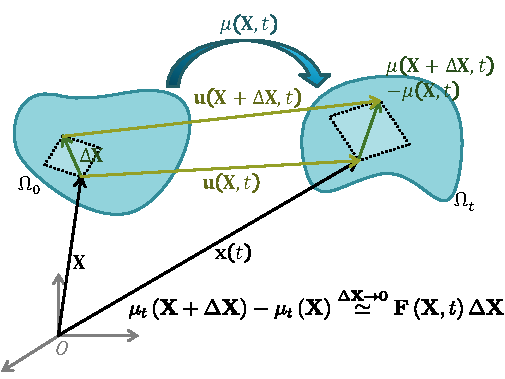
\includegraphics{images/III.6.2.pdf}
    \caption{在参考位置$\mathbf{X}$和$\mathbf{X}+\Delta\mathbf{X}$的两物质点,在形变$\mu_t$后的当前位置差别,是映射$\mu\left(\Delta\mathbf{X},t\right)\equiv\mu_t\left(\mathbf{X}\right)$关于$\mathbf{X}$的增量。由形变梯度张量$\mathbf{F}$的定义,当$\Delta\mathbf{X}\to\mathbf{0}$时$\mu_t$的增量可由$\mathbf{F}\Delta\mathbf{X}$近似。因此$\mathbf{F}\left(\mathbf{X},t\right)$实际表示在参考位置$\mathbf{X}$的邻域的形变。图中还标出了位移场$\mathbf{u}\left(\mathbf{X},t\right)$,根据向量关系可知$\mathrm{d}_{\mathbf{X}}\mathbf{u}\left(\mathbf{X},t\right)=\mathbf{F}-\mathbf{I}$。}
    \label{fig:III.6.2}
\end{figure}

一般地,关于参考构型不同点$\mathbf{X}$的邻域可能发生不同类型和程度的形变。对于连续物体,我们可以用形变映射的微分来表示每一点$\mathbf{X}$邻域的形变:
\[\mu_t\left(\mathbf{X}+\Delta\mathbf{X}\right)-\mu_t\left(\mathbf{X}\right)=\mathbf{F}\left(\mathbf{X},t\right)\Delta\mathbf{X}+o\left(\left\|\Delta\mathbf{x}\right\|\right)\]
其中
\[\mathbf{F}\left(\mathbf{X},t\right)\equiv \mathrm{d}_{\mathbf{X}^\prime=\mathbf{X}}\mu_t\left(\mathbf{X}^\prime\right)\]
是函数$\mu_t$在$\mathbf{X}$处的导数,它是平移空间$\mathcal{V}$上的线性算符。由于$\mu_t$是任意所需阶光滑的,由定理\ref{thm:II.4.12}的推论,$\mathrm{det}\mathbf{F}\neq 0$,即$\mathbf{F}\left(\mathbf{X},t\right)$的取值总是可逆线性算符。

由$\mathbf{F}$所对应的微分式和图\ref{fig:III.6.2}可知,线性算符$\mathbf{F}\left(\mathbf{X},t\right)$实际表示在参考位置$\mathbf{X}$的小邻域发生形变。一个线性算符如何表示形变,可回顾\S\ref{sec:II.3.3}。

形变梯度张量与位移场的梯度只相关一个单位算符$\mathbf{I}$。由位移场的微分:
\begin{align*}
    \mathbf{u}\left(\mathbf{X}+\Delta\mathbf{X}\right)-\mathbf{u}\left(\mathbf{X}\right) & =\mathrm{d}_{\mathbf{X}}\mathbf{u}\left(\mathbf{X}\right)\Delta\mathbf{X}+o\left(\left\|\Delta\mathbf{X}\right\|\right)                      \\
                                                                                         & =\mu_t\left(\mathbf{X}+\Delta\mathbf{X}\right)-\left(\mathbf{X}+\Delta\mathbf{X}\right)-\left[\mu_t\left(\mathbf{X}\right)-\mathbf{X}\right] \\
                                                                                         & =\mu_t\left(\mathbf{X}+\Delta\mathbf{X}\right)-\Delta\mathbf{X}                                                                              \\
                                                                                         & =\mathbf{F}\left(\mathbf{X},t\right)\Delta\mathbf{X}+o\left(\left\|\Delta\mathbf{X}\right\|\right)
\end{align*}
可得$\mathrm{d}_{\mathbf{X}}\mathbf{u}\left(\mathbf{X},t\right)=\mathbf{F}\left(\mathbf{X},t\right)-\mathbf{I}$。

在$\mathcal{E}$的基本直角坐标系下,$\mathbf{F}\left(\mathbf{X},t\right)$的坐标矩阵是
\[\left(\begin{array}{ccc}\frac{\partial \eta}{\partial X_1} & \frac{\partial\eta}{\partial X_2}  & \frac{\partial\eta}{\partial X_3}  \\
             \frac{\partial\xi}{\partial X_1}        & \frac{\partial\xi}{\partial X_2}   & \frac{\partial\xi}{\partial X_3}   \\
             \frac{\partial\zeta}{\partial X_1}      & \frac{\partial\zeta}{\partial X_2} & \frac{\partial\zeta}{\partial X_3}\end{array}\right)\]

一般地,$\mathbf{F}\left(\mathbf{X},t\right)$的取值依赖是依赖参考位置$\mathbf{X}$的。若$\mathbf{F}\left(\mathbf{X},t\right)$不依赖$\mathbf{X}$,则称所关心物体的形变$\mu_t$是\emph{均匀(homogeneous)}的。特别地,当$\mathbf{F}\equiv\mathbf{I}$时,所关心的物体的每个物质点都只发生大小和方向相同的位移(位移场梯度为零)。

由极分解定理\ref{thm:II.2.37},结合$\mathbf{F}$的值总是可逆算符,可知形变梯度张量总有极分解
\[\mathbf{F}=\mathbf{RU}=\mathbf{VR}\]
其中$\mathbf{R}\left(\mathbf{X},t\right)$的值是正交算符,$\mathbf{U}\left(\mathbf{X},t\right)$、$\mathbf{V}\left(\mathbf{X},t\right)$的值是非负对称算符,分别称为\emph{右、左拉伸张量(right/left stretch tensor)},且有$\mathbf{V}=\mathbf{R}^\intercal\mathbf{UR}$。这时,\S\ref{sec:II.3.3}的内容就可以更加直接地用于理解$\mathbf{F}$。若可以简单说正交算符表示刚体旋转、对称算符表示3轴拉伸、算符的映射复合是形变的叠加操作,那么极分解定理告诉我们任何一个局域的形变都是一个局域的3轴拉伸和一个局域的刚体旋转的叠加。由
\[\mathrm{det}\mathbf{F}=\mathrm{det}\left(\mathbf{RU}\right)=\mathrm{det}\left(\mathbf{VR}\right)\]
以及正交算符性质$\mathrm{det}\mathbf{R}=\pm 1$和规定$\mathrm{det}\mathbf{F}\neq 0$可知,$\mathrm{det}\mathbf{U}=\mathbf{det}\mathbf{V}>0$。由于与\S\ref{sec:II.3.4}最后所述类似的理由,物体无法发生镜象翻转的形变\footnote{右手无法形变为左手。},因此在连续介质力学中$\mathbf{R}$只允许为行列式等于1的正交算符。这一规定往往等价地表述为:$\mathrm{det}\mathbf{F}>0$。

由于$\mathbf{U}$或$\mathbf{V}$是正定对称张量且它们正交等价,故它们有相同的一组特征值$\lambda_1,\lambda_2,\lambda_3$,称为\emph{主拉伸比(principal stretch ratios)}。$\mathbf{U}$或$\mathbf{V}$的相应的主轴称\emph{主拉伸方向(principal stretch directions)}。

如果我们认为,一个物体在运动中除刚体平动外,只发生了刚体旋转,则“形变为零”,那么形变梯度张量$\mathbf{F}=\mathbf{I}$并不意味着这种意义上的“无形变”,因为至少当一个物体发生由$\mathbf{R}$描述的刚体旋转时,$\mathbf{F}=\mathbf{R}\neq\mathbf{I}$。满足我们的这一意图的形变的量度应该是拉伸张量$\mathbf{U}$或$\mathbf{V}$。我们对上述意义下的“零形变”的关注来自对弹性材料的直观感受。我们对弹性材料直观体验是,材料产生应力是由于材料形成了应变;无应变则无应力\footnote{在后面的章节将看到,严格定义下的应力并不依赖应变,更不一定在无应变时为零。}。因此我们可以说,$\mathbf{U}$或$\mathbf{V}$是\emph{应变量度(strain measures)}。一切仅由三个主拉伸方向和主拉伸比确定的线性算符值函数都可等价地作为应变量度\cite[Sect.32]{Truesdell1960}。比如由$\mathbf{U}$或$\mathbf{V}$分别定义的
\begin{align*}
    \mathbf{C}\left(\mathbf{X},t\right) & \equiv\mathbf{U}^2\left(\mathbf{X},t\right)                                                    \\
                                        & =\left(\mathbf{F}\left(\mathbf{X},t\right)\right)^\intercal\mathbf{F}\left(\mathbf{X},t\right)
\end{align*}
称\emph{右柯西--格林应变张量(right Cauchy--Green strain tensor)},
\begin{align*}
    \mathbf{B}\left(\mathbf{X},t\right) & \equiv\mathbf{V}^2\left(\mathbf{X},t\right)                                                    \\
                                        & =\mathbf{F}\left(\mathbf{X},t\right)\left(\mathbf{F}\left(\mathbf{X},t\right)\right)^\intercal
\end{align*}
称\emph{左柯西--格林应变张量(left Cauchy--Green strain tensor)}。当且仅当主拉伸比取值都为1时,$\mathbf{U}=\mathbf{V}=\mathbf{C}=\mathbf{B}=\mathbf{I}$。故物体存在的刚体平动或转动都不影响上述应变量度的取值。我们希望在相同的条件下,应变量度的取值为“零”,故再定义
\begin{align*}
    \mathbf{E}\left(\mathbf{X},t\right) & \equiv\frac{1}{2}\left(\mathbf{C}\left(\mathbf{X},t\right)-\mathbf{I}\right)                   \\
    \mathbf{e}\left(\mathbf{X},t\right) & \equiv\frac{1}{2}\left(\mathbf{I}-\left(\mathbf{B}\left(\mathbf{X},t\right)^{-1}\right)\right)
\end{align*}
分别称\emph{格林应变张量(Green strain tensor)}和\emph{阿尔曼西应变张量(Almansi strain tensor)}\footnote{注意区分两种不同意义的“逆”的记号:$\mathbf{B}^{-1}\left(\mathbf{X},t\right)$表示关于自变量$\left(\mathbf{X},t\right)$的逆映射,$\left(\mathbf{B}\left(\mathbf{X},t\right)\right)^{-1}$表示作为函数值的线性算符的逆变换。}。









\end{document}